\section{Metric Reconstruction}
\label{sec:essmatrix}

You will compute the camera matrices and triangulate the 2D points to obtain the 3D scene structure. To obtain the Euclidean scene structure, first convert the fundamental matrix $\F$ to an essential matrix $\E$. Examine the lecture notes and the textbook to find out how to do this when the internal camera calibration matrices $\K_1$ and $\K_2$ are known; these are provided in \texttt{data/intrinsics.npz}.

\subparagraph*{Q3.1}\points{5}
Complete the function \texttt{essentialMatrix} in \texttt{q3\_1\_essential\_matrix.py} to compute the essential matrix $\E$ given $\F$, $\K_1$ and $\K_2$ with the signature:
\begin{center}
    \texttt{E = essentialMatrix(F, K1, K2)}
\end{center}

\deliver{
\textbf{Output:} Save your estimated $\E$ using $\F$ from the eight-point algorithm to \texttt{q3\_1.npz}.\\
\textbf{In your write-up: }
\begin{itemize}
    \item Write your estimated $\textbf{E}$
    \item Include the code snippet of \texttt{essentialMatrix} function
\end{itemize}
}

\begin{your_solution}[title=Q3.1,height=12.5cm,width=\linewidth]
	As in the output: $./q3\_1.npz$, the recovered E is: 
	\newline
	
	$\begin{pmatrix}
	-5.06923074e^{-01} &  6.86542875e^{+01} & -3.71961318e^{+02}\\
	2.97106690e^{+01}  & -1.54718732e^{+00} &  9.68232032e^{+00}\\
	3.72990948e^{+02}  &  2.98549953e^{+00} &  1.50354471e^{-01}
	\end{pmatrix}$
	\newline
	
The following \autoref{fig:Q3_1_cns} shows the code snippet of the q3\_1\_essential\_matrix.py:
\newline

%\begin{minipage}{1\linewidth}
	%\centering
	%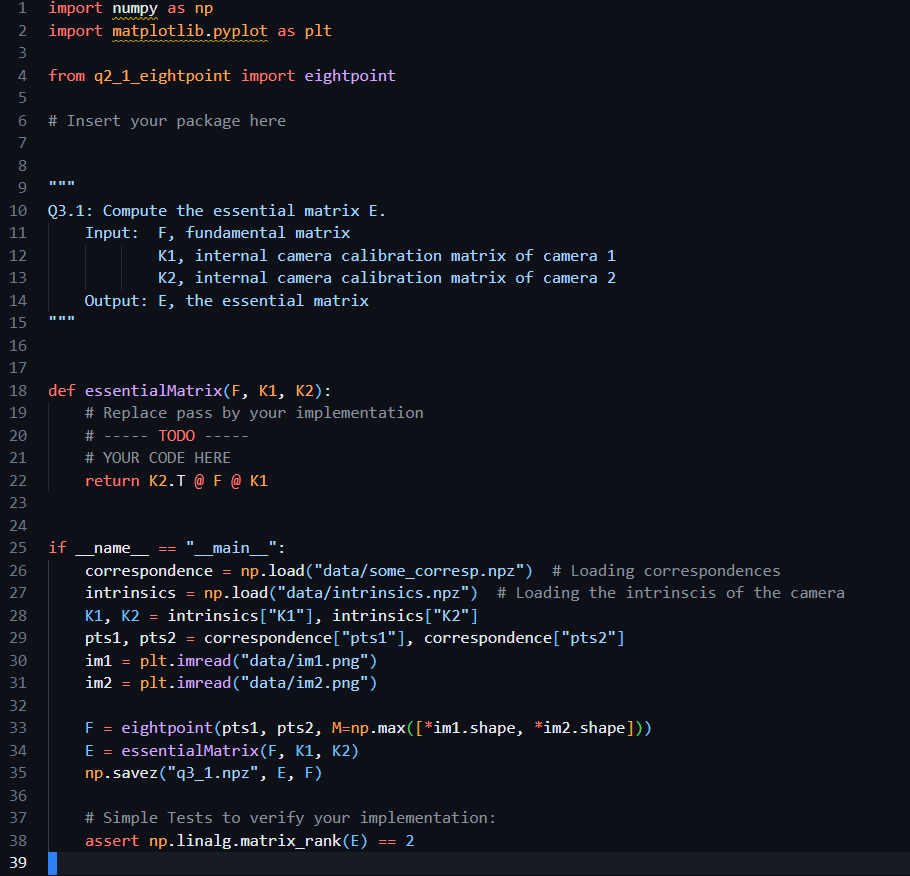
\includegraphics[width=0.5\linewidth]{../Q3_1_cns.png}
	%\refstepcounter{figure}  % Increment the figure counter
	%\textbf{Figure \ref{fig:Q3_1_cns}:} Code Snippet  % Manually add a caption/title
	%\label{fig:Q3_1_cns}         % Label for referencing	
%\end{minipage}	

\begin{minipage}{1\linewidth}
	\centering
	\hspace{0.12\linewidth} 
	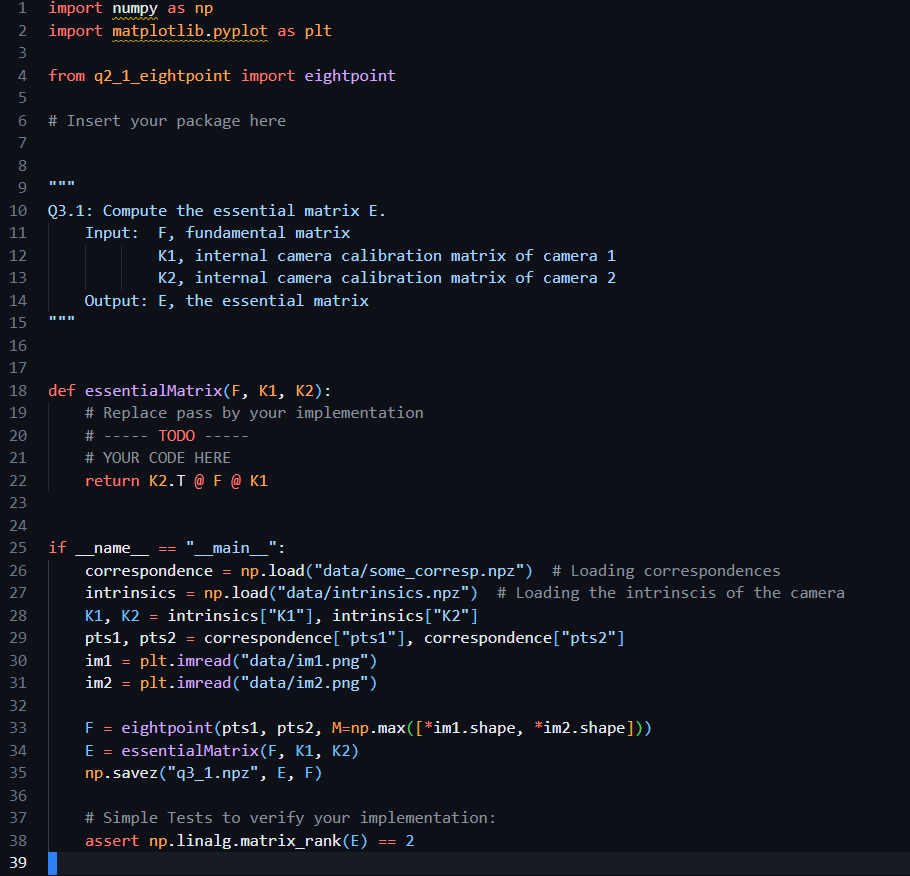
\includegraphics[width=0.5\linewidth]{../Q3_1_cns.png}  % Adjust the width to 50% of the line width
	\refstepcounter{figure}  % Increment the figure counter
	\newline
	\textbf{Figure \thefigure:} Code Snippet % Manually add a caption/title
	\label{fig:Q3_1_cns}  % Label for referencing
\end{minipage}

\end{your_solution}

\hfill\\

Given an essential matrix, it is possible to retrieve the projective camera matrices $\M_1$ and $\M_2$ from it.  Assuming $\M_1$ is fixed at $[\I,0]$, $\M_2$ can be retrieved up to a scale and four-fold rotation ambiguity. For details on recovering $\M_2$, see section 11.3 in Szeliski. We have provided you with the function \texttt{camera2} in \texttt{python/helper.py} to recover the four possible $\M_2$ matrices given $\E$.

\textbf{Note: } The matrices $\M1$ and $\M2$ here are of the form: 
$\M_1 = \begin{bmatrix}\I | 0\end{bmatrix} $ and $\M_2 = \begin{bmatrix}\R | \t\end{bmatrix} $.

\subparagraph*{Q3.2}\points{10}
Using the above, complete the function \texttt{triangulate} in \texttt{q3\_2\_triangulate.py} to triangulate a set of 2D coordinates in the image to a set of 3D points with the signature:
\begin{center}
    \texttt{[w, err] = triangulate(C1, pts1, C2, pts2)}
\end{center}
where \texttt{pts1} and \texttt{pts2} are the $N \times 2$ matrices with the 2D image coordinates and \texttt{w} is an $N \times 3$ matrix with the corresponding 3D points per row.  \texttt{C1} and \texttt{C2} are the $3 \times 4$ camera matrices. Remember that you will need to multiply the given intrinsics matrices with your solution for the canonical camera matrices to obtain the final camera matrices. Various methods exist for triangulation -
probably the most familiar for you is based on least squares (see \cite{szeliski2022computer} Chapter 7 if you want to learn about other methods).

For each point $i$, we want to solve for 3D coordinates $\w_i = \begin{bmatrix}x_i, y_i, z_i\end{bmatrix}^T$, such that when they are projected back to the two images, they are close to the original 2D points. To project the 3D coordinates back to 2D images, we first write $\w_i$ in homogeneous coordinates, and compute $\mathbf{C}_1 \tilde{\w_i}$ and $\mathbf{C}_2 \tilde{\w_i}$ to obtain the 2D homogeneous coordinates projected to camera $1$ and camera $2$, respectively.

For each point $i$, we can write this problem in the following form:
\begin{align*}
\mathbf{A}_i\w_i = 0,
\end{align*}
where $\mathbf{A}_i$ is a $4\times 4$ matrix, and $\tilde{\w_i}$ is a $4\times 1$ vector of the 3D coordinates in the homogeneous form. Then, you can obtain the homogeneous least-squares solution (discussed in class) to solve for each $\w_i$.

Once you have implemented triangulation, check the performance by looking at the reprojection error:  
\begin{align*}
\texttt{err} = \sum_i \|\x_{1i}, \widehat{\x_{1i}}\|^2 + \|\x_{2i}, \widehat{\x_{2i}}\|^2    
\end{align*}
where $\widehat{\x_{1i}} = Proj(\mathbf{C}_1, \w_i)$ and $\widehat{\x_{2i}} = Proj(\mathbf{C}_2, \w_i)$. You should see an error less than 500. Ours is around 350. 

\textbf{Note: } \texttt{C1} and \texttt{C2} here are projection matrices of the form:
$\mathbf{C}_1 = \mathbf{K}_1\mathbf{M}_1 = \mathbf{K}_1 \begin{bmatrix}
\I | 0
\end{bmatrix} $ and $\mathbf{C}_2 =  \mathbf{K}_2\mathbf{M}_2 = \mathbf{K}_2 \begin{bmatrix}
\R | \t
\end{bmatrix}$.

\deliver{
\textbf{In your write-up:} 
\begin{itemize}
    \item Write down the expression for the matrix $\mathbf{A}_i$ for triangulating a pair of 2D coordinates in the image to a 3D point.
    \item Include the code snippet of \texttt{triangulate} function.
\end{itemize}
}

\begin{your_solution}[title=Q3.2,height=22.5cm,width=\linewidth]
Assume that $\mathbf{w}_i = \begin{bmatrix} x_i \\ y_i \\ z_i \end{bmatrix}$ is the 3D coordinates at point i, and $\tilde{\mathbf{w}}_i = \begin{bmatrix} x_i \\ y_i \\ z_i \\ 1 \end{bmatrix}$ is its homogeneous coordinate. Besides, $u_1 = \lambda_1\begin{bmatrix} u_{xi_{1}} \\ u_{yi_{1}} \\ 1 \end{bmatrix}$ is the 2D projected homogeneous coordinates on camera1 and $u_2 = \lambda_2\begin{bmatrix} u_{xi_{2}} \\ u_{yi_{2}} \\ 1 \end{bmatrix}$ is the 2D projected homogeneous coordinates on camera2. Let us define the C1 and C2 camera matrix as the following:
\begin{align}
	C1 = \begin{bmatrix}
		c_{1_{11}} & c_{1_{12}} & c_{1_{13}} & c_{1_{14}} \\
		c_{1_{21}} & c_{1_{22}} & c_{1_{23}} & c_{1_{24}} \\
		c_{1_{31}} & c_{1_{32}} & c_{1_{33}} & c_{1_{34}}
	\end{bmatrix} \\
	C2 = \begin{bmatrix}
	c_{2_{11}} & c_{2_{12}} & c_{2_{13}} & c_{2_{14}} \\
	c_{2_{21}} & c_{2_{22}} & c_{2_{23}} & c_{2_{24}} \\
	c_{2_{31}} & c_{2_{32}} & c_{2_{33}} & c_{2_{34}}
	\end{bmatrix}
	%\lambda_1 \begin{bmatrix} x_1 \\ y_1 \\ 1 \end{bmatrix} = K(R_1 \begin{bmatrix} X_P \\ Y_P \\ Z_P \end{bmatrix}) + t_1 \\
	%\lambda_2 \begin{bmatrix} x_2 \\ y_2 \\ 1 \end{bmatrix} = K(R_2 \begin{bmatrix} X_P \\ Y_P \\ Z_P \end{bmatrix}) + t_2
\end{align}
Then, we have the following two equations:
\begin{align}
	 \lambda_1\begin{bmatrix} u_{xi_{1}} \\ u_{yi_{1}} \\ 1 \end{bmatrix} = \begin{bmatrix}
		c_{1_{11}} & c_{1_{12}} & c_{1_{13}} & c_{1_{14}} \\
		c_{1_{21}} & c_{1_{22}} & c_{1_{23}} & c_{1_{24}} \\
		c_{1_{31}} & c_{1_{32}} & c_{1_{33}} & c_{1_{34}}
	\end{bmatrix} \begin{bmatrix} x_i \\ y_i \\ z_i \\ 1 \end{bmatrix} \\
	 \lambda_2\begin{bmatrix} u_{xi_{2}} \\ u_{yi_{2}} \\ 1 \end{bmatrix} = \begin{bmatrix}
		c_{2_{11}} & c_{2_{12}} & c_{2_{13}} & c_{2_{14}} \\
		c_{2_{21}} & c_{2_{22}} & c_{2_{23}} & c_{2_{24}} \\
		c_{2_{31}} & c_{2_{32}} & c_{2_{33}} & c_{2_{34}}
	\end{bmatrix} \begin{bmatrix} x_i \\ y_i \\ z_i \\ 1 \end{bmatrix}
\end{align}
After multiplying both equation (6) and (7) out, dividing x and y coordinates by the z coordinate, and rearranging the equations, we get the following equation:
\begin{align}
	\begin{bmatrix}
		c_{1_{11}}-u_{xi_{1}}c_{1_{31}} & c_{1_{12}}-u_{xi_{1}}c_{1_{32}} & c_{1_{13}}-u_{xi_{1}}c_{1_{33}} & c_{1_{14}}-u_{xi_{1}}c_{1_{34}} \\
		c_{1_{21}}-u_{yi_{1}}c_{1_{31}} & c_{1_{22}}-u_{yi_{1}}c_{1_{32}} & c_{1_{23}}-u_{yi_{1}}c_{1_{33}} & c_{1_{24}}-u_{yi_{1}}c_{1_{34}} \\
		c_{2_{11}}-u_{xi_{2}}c_{2_{31}} & c_{2_{12}}-u_{xi_{2}}c_{2_{32}} & c_{2_{13}}-u_{xi_{2}}c_{2_{33}} & c_{2_{14}}-u_{xi_{2}}c_{2_{34}} \\
		c_{2_{21}}-u_{yi_{2}}c_{2_{31}} & c_{2_{22}}-u_{yi_{2}}c_{2_{32}} & c_{2_{23}}-u_{yi_{2}}c_{2_{33}} & c_{2_{24}}-u_{yi_{2}}c_{2_{34}}
	\end{bmatrix} \begin{bmatrix} x_i \\ y_i \\ z_i \\ 1 \end{bmatrix} = 0
\end{align}
Accordingly, we have A matrix: \newline
\begin{align}
A = \begin{bmatrix}
	c_{1_{11}}-u_{xi_{1}}c_{1_{31}} & c_{1_{12}}-u_{xi_{1}}c_{1_{32}} & c_{1_{13}}-u_{xi_{1}}c_{1_{33}} & c_{1_{14}}-u_{xi_{1}}c_{1_{34}} \\
	c_{1_{21}}-u_{yi_{1}}c_{1_{31}} & c_{1_{22}}-u_{yi_{1}}c_{1_{32}} & c_{1_{23}}-u_{yi_{1}}c_{1_{33}} & c_{1_{24}}-u_{yi_{1}}c_{1_{34}} \\
	c_{2_{11}}-u_{xi_{2}}c_{2_{31}} & c_{2_{12}}-u_{xi_{2}}c_{2_{32}} & c_{2_{13}}-u_{xi_{2}}c_{2_{33}} & c_{2_{14}}-u_{xi_{2}}c_{2_{34}} \\
	c_{2_{21}}-u_{yi_{2}}c_{2_{31}} & c_{2_{22}}-u_{yi_{2}}c_{2_{32}} & c_{2_{23}}-u_{yi_{2}}c_{2_{33}} & c_{2_{24}}-u_{yi_{2}}c_{2_{34}}
\end{bmatrix}
\end{align}
\end{your_solution}

\begin{your_solution}[title=Q3.2 continued,height=15.5cm,width=\linewidth]
The following \autoref{fig:Q3_2_cns} shows the code snippet of triangulate() in the q3\_2triangulate.py:
\newline

\begin{minipage}{1\linewidth}
	\centering
	\hspace{0.12\linewidth} 
	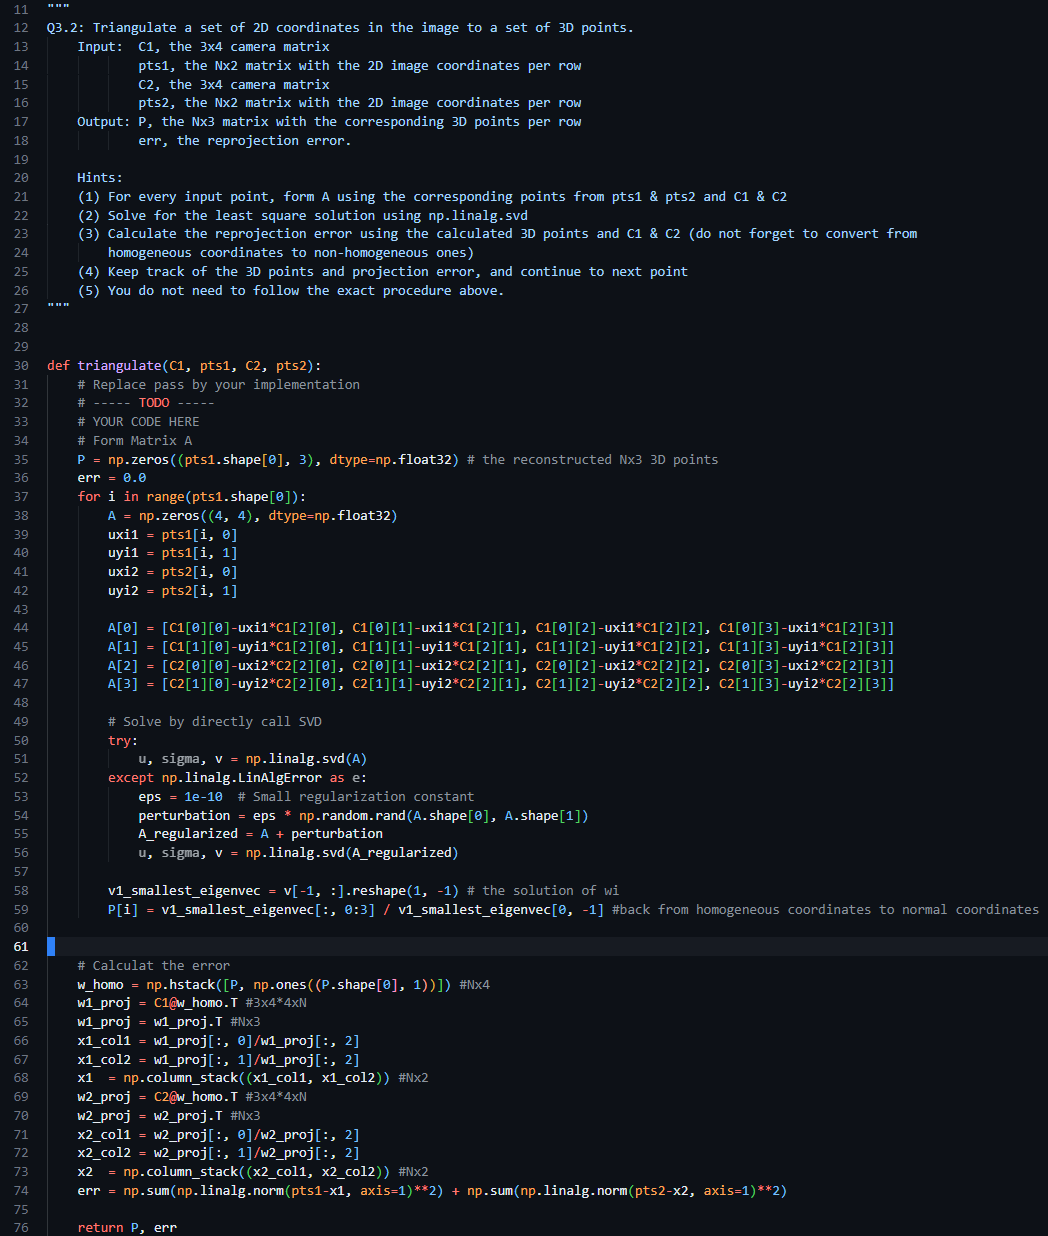
\includegraphics[width=0.7\linewidth]{../Q3_2_cns.png}  % Adjust the width to 50% of the line width
	\refstepcounter{figure}  % Increment the figure counter
	\newline
	\textbf{Figure \thefigure:} Code Snippet % Manually add a caption/title
	\label{fig:Q3_2_cns}  % Label for referencing
\end{minipage}
\end{your_solution}

\subparagraph*{Q3.3}\points{10}
Complete the function \texttt{findM2} in \texttt{q3\_2\_triangulate.py} to obtain the correct \texttt{M2} from \texttt{M2s} by testing the four solutions through triangulations.\\Use the correspondences from \texttt{data/some\_corresp.npz}.

\deliver{
\textbf{Output:} Save the correct \texttt{M2},
the corresponding \texttt{C2}, and 3D points \texttt{P} to \texttt{q3\_3.npz}.\\ 
\textbf{In your writeup:} Include the code snippet of \texttt{findM2} function.
}

\begin{your_solution}[title=Q3.3,height=14.5cm,width=\linewidth]
	The following \autoref{fig:Q3_3_cns} shows the code snippet of findM2() in the q3\_2triangulate.py:
	\newline
	
	\begin{minipage}{1\linewidth}
		\centering
		\hspace{0.12\linewidth} 
		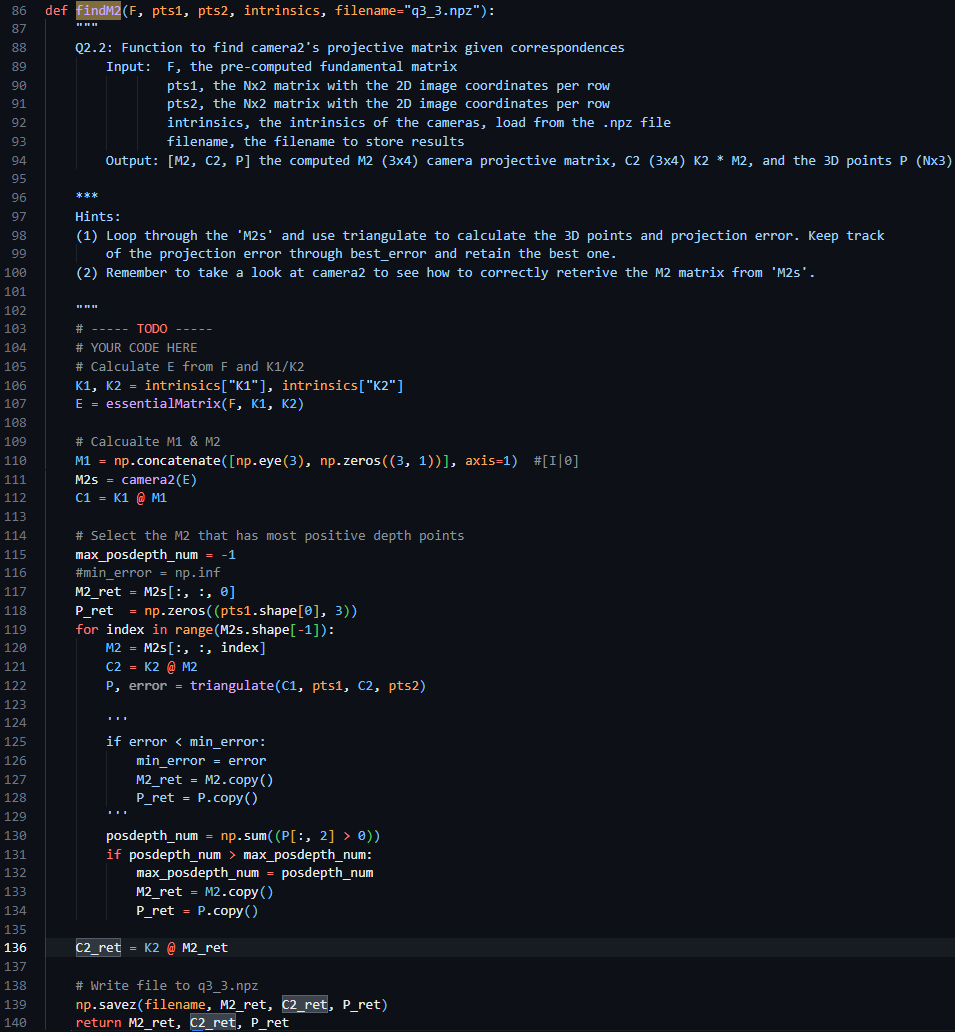
\includegraphics[width=0.7\linewidth]{../Q3_3_cns.png}  % Adjust the width to 50% of the line width
		\refstepcounter{figure}  % Increment the figure counter
		\newline
		\textbf{Figure \thefigure:} Code Snippet % Manually add a caption/title
		\label{fig:Q3_3_cns}  % Label for referencing
	\end{minipage}
\end{your_solution}

